\documentclass{article}

\usepackage{fancyhdr}
\usepackage{extramarks}
\usepackage{amsmath}
\usepackage{amsthm}
\usepackage{amsfonts}
\usepackage{tikz}
\usepackage[plain]{algorithm}
\usepackage{algpseudocode}
\usepackage{enumitem}
\usepackage{mathtools}
\usepackage{amssymb}
\usetikzlibrary{automata,positioning}
\usepackage{pgfplots}
\usepackage{graphicx}


%
% Basic Document Settings
%

\topmargin=-0.45in
\evensidemargin=0in
\oddsidemargin=0in
\textwidth=6.5in
\textheight=9.0in
\headsep=0.25in

\linespread{1.1}

\pagestyle{fancy}
\lhead{\hmwkClass\ \hmwkTitle}
\rhead{\hmwkAuthorName}
\lfoot{\lastxmark}
\cfoot{\thepage}

\renewcommand\headrulewidth{0.4pt}
\renewcommand\footrulewidth{0.4pt}

\setlength\parindent{0pt}

%
% Added stuff
%

\DeclarePairedDelimiter\abs{\lvert}{\rvert}
\setenumerate[0]{label={(\alph*)}}

\pgfplotsset{my style/.append style={axis x line=middle, axis y line=
           middle, xlabel={$x$}, ylabel={$y$}, axis equal }}

%
% Create Problem Sections
%

\newcommand{\enterProblemHeader}[1]{
    \nobreak\extramarks{}{Problem \arabic{#1} continued on next page\ldots}\nobreak{}
    \nobreak\extramarks{Problem \arabic{#1} (continued)}{Problem \arabic{#1} continued on next page\ldots}\nobreak{}
}

\newcommand{\exitProblemHeader}[1]{
    \nobreak\extramarks{Problem \arabic{#1} (continued)}{Problem \arabic{#1} continued on next page\ldots}\nobreak{}
    \stepcounter{#1}
    \nobreak\extramarks{Problem \arabic{#1}}{}\nobreak{}
}

\setcounter{secnumdepth}{0}
\newcounter{partCounter}
\newcounter{homeworkProblemCounter}
\setcounter{homeworkProblemCounter}{1}
\nobreak\extramarks{Problem \arabic{homeworkProblemCounter}}{}\nobreak{}

%
% Homework Problem Environment
%
% This environment takes an optional argument. When given, it will adjust the
% problem counter. This is useful for when the problems given for your
% assignment aren't sequential. See the last 3 problems of this template for an
% example.
%
\newenvironment{homeworkProblem}[1][-1]{
    \ifnum#1>0
        \setcounter{homeworkProblemCounter}{#1}
    \fi
    \section{Problem \arabic{homeworkProblemCounter}}
    \setcounter{partCounter}{1}
    \enterProblemHeader{homeworkProblemCounter}
}{
    \exitProblemHeader{homeworkProblemCounter}
}

%
% Homework Details
%   - Title
%   - Due date
%   - Class
%   - Section/Time
%   - Instructor
%   - Author
%

\newcommand{\hmwkTitle}{Worksheet\ \#8 - Matrix Factorization}
\newcommand{\hmwkDueDate}{March 6, 2017}
\newcommand{\hmwkClass}{DSE 210}
\newcommand{\hmwkClassTime}{}
\newcommand{\hmwkClassInstructor}{Professor: A. Enis \c{C}etin}
\newcommand{\hmwkClassTA}{Teaching Assistant: Shivani Agrawal}
\newcommand{\hmwkAuthorName}{\textbf{Joshua Wilson} \and \textbf{A53228518}}

%
% Title Page
%

\title{
    \vspace{2in}
    \textmd{\textbf{\hmwkClass:\ \hmwkTitle}}\\
    \vspace{0.1in}\large{\textit{\hmwkClassInstructor}}\\
    \vspace{0.1in}\large{\textit{\hmwkClassTA}}
    \vspace{3in}
}

\author{\hmwkAuthorName}
\date{}

\renewcommand{\part}[1]{\textbf{\large Part \Alph{partCounter}}\stepcounter{partCounter}\\}

%
% Various Helper Commands
%

% Useful for algorithms
\newcommand{\alg}[1]{\textsc{\bfseries \footnotesize #1}}

% For derivatives
\newcommand{\deriv}[1]{\frac{\mathrm{d}}{\mathrm{d}x} (#1)}

% For partial derivatives
\newcommand{\pderiv}[2]{\frac{\partial}{\partial #1} (#2)}

% Integral dx
\newcommand{\dx}{\mathrm{d}x}

% Alias for the Solution section header
\newcommand{\solution}{\textbf{\large Solution}}

% Probability commands
\newcommand{\E}{\mathrm{E}}
\newcommand{\Var}{\mathrm{Var}}
\newcommand{\Cov}{\mathrm{Cov}}
\newcommand{\Bias}{\mathrm{Bias}}
\newcommand*{\Perm}[2]{{}_{#1}\!P_{#2}}%
\newcommand*{\Comb}[2]{{}_{#1}C_{#2}}%
\newcommand\given[1][]{\:#1\vert\:}
\newcommand{\norm}[1]{\left\lVert#1\right\rVert}
\DeclareMathOperator*{\argmax}{arg\,max}

\begin{document}

\maketitle

\pagebreak

\begin{homeworkProblem}

$\Bigg\{ \begin{bmatrix}\ 3 \\ 4 \\ 0 \end{bmatrix}, \begin{bmatrix} 4 \\ -3 \\ 0 \end{bmatrix}, \begin{bmatrix} 0 \\ 0 \\ 1 \end{bmatrix} \Bigg\}$ is not an orthonormal basis, because 
$\norm{\begin{bmatrix}\ 3 \\4 \\0 \end{bmatrix}} = \sqrt{3^2 + 4^2 + 0^2} = \sqrt{25} = 5 \neq 1$.
\end{homeworkProblem}

\begin{homeworkProblem}
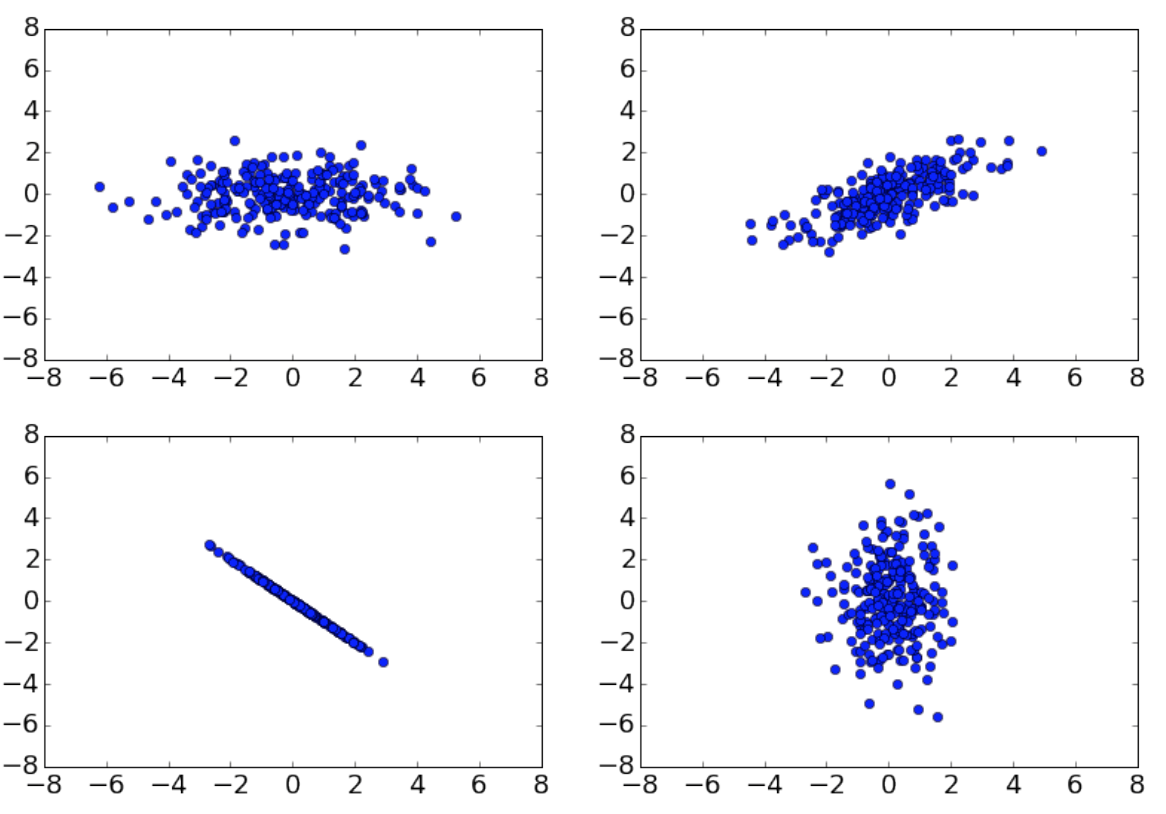
\includegraphics[width=\linewidth]{Worksheet8Problem2}
\end{homeworkProblem}

\begin{homeworkProblem}
\begin{enumerate}
\item
\begin{itemize}
\item $U \text{ is }p \times 2$
\item $U^T \text{ is }2 \times p$
\item $UU^T \text{ is }p \times p$
\item $u_1u_1^T \text{ is }p \times p$
\end{itemize}
\item
\begin{itemize}
\item $x \mapsto (u_1 \cdot x, u_2 \cdot x)$ is the projection of $x$ onto the 2-dimensional subspace defined by $u_1, u_2$
\item $x \mapsto (u_1 \cdot x) u_1 + (u_2 \cdot x) u_2$ is the projection of $x$ as a p-dimensional vector onto the subspace defined by $u_1, u_2$
\item $x \mapsto U^T x$ is the projection of $x$ on to the 2-dimensional subspace defined by $u_1, u_2$ (same as $x \mapsto (u_1 \cdot x, u_2 \cdot x)$)
\item $x \mapsto UU^T x$ is the projection of $x$ as a p-dimensional vector onto the subspace defined by $u_1, u_2$ (same as $x \mapsto (u_1 \cdot x) u_1 + (u_2 \cdot x) u_2$)
\end{itemize}
\end{enumerate}
\end{homeworkProblem}

\begin{homeworkProblem}
See Worksheet7\_8.ipynb notebook at https://github.com/mas-dse/jsw037/tree/master/DSE210.
\end{homeworkProblem}

\end{document}




